% ACL 2024 style submission
% Use: pdflatex fleek_paper.tex (requires acl.sty from ACL Anthology)
% Overleaf template: https://www.overleaf.com/latex/templates/acl-2023-proceedings-template/qjdgcrdwcnwp

\documentclass[11pt]{article}

% --- ACL style ---
% Download acl.sty from https://github.com/acl-org/acl-style-files
% and place in same directory, or use the Overleaf ACL template.
\usepackage[review]{acl}

% --- Standard packages ---
\usepackage{times}
\usepackage{latexsym}
\usepackage[T1]{fontenc}
\usepackage[utf8]{inputenc}
\usepackage{microtype}
\usepackage{inconsolata}
\usepackage{graphicx}
\usepackage{booktabs}
\usepackage{amsmath}
\usepackage{multirow}
\usepackage{xcolor}
\usepackage{soul}           % for \hl{} highlighting of TODOs
\usepackage{hyperref}
\usepackage{url}

% --- TODO command ---
\newcommand{\todo}[1]{\hl{\textbf{TODO:} #1}}

% --- JSON embedding command ---
\usepackage{listings}
\usepackage{xcolor}

\lstdefinelanguage{json}{
    basicstyle=\ttfamily\small,
    numbers=left,
    numberstyle=\tiny\color{gray},
    stepnumber=1,
    numbersep=5pt,
    showstringspaces=false,
    breaklines=true,
    frame=single,
    rulecolor=\color{black!30},
    backgroundcolor=\color{gray!8},
    stringstyle=\color{teal},
    keywordstyle=\color{blue},
    commentstyle=\color{gray},
    morestring=[b]",
}

% --- Paper metadata ---
\title{LLMs Can't Keep Up with Language That's on Fleek\\
{\large How Training Data Age Shapes (and Freezes) Model Vocabulary}}

% Remove author block for anonymous review; fill in for camera-ready.
% \author{Author Name \\ Institution \\ \texttt{email@example.com}}

\begin{document}

\maketitle

% ============================================================
\begin{abstract}
Large language models trained on internet-sourced corpora inherit not just the knowledge but the temporal language patterns of their training data. Because training data timestamping is not a factor at model training time, LLMs likely reflect an undifferentiated blend of language from across their entire corpus window rather than prioritizing recently popular language. This paper investigates whether LLMs demonstrate temporal awareness of slang and informal vocabulary, and whether their language usage is frozen relative to the pace of real-world linguistic change. We propose and execute
experiments using Common Crawl dump analysis and LLM output probing to surface this effect, and discuss implications for the future of training data and potential mitigations.

\todo{Verify the core thesis holds after initial experiments --- revise abstract accordingly.}
\end{abstract}

% ============================================================
\section{Introduction}

\subsection{Motivation: Training Data Growth and Its Limits}

Large language models have scaled rapidly on the back of ever-growing
internet text corpora. The relationship between data volume and model
capability is well-established: \citet{hoffmann2022chinchilla}
demonstrate that compute-optimal training requires scaling training
tokens proportionally with model parameters (\textit{Chinchilla}), and
subsequent work has confirmed that data scale remains a primary lever
for capability improvements. Historically, the added volume of available
training data has grown year-over-year, making recency a less pressing
concern. However, this dynamic is beginning to shift.

LLM-generated text is increasingly prevalent online, threatening
  to contaminate future training pools with model outputs rather than
  authentic human language. \citet{shumailov2023curse} show that
  training on model-generated content causes irreversible defects in the
  resulting models, where tails of the original content distribution
  disappear --- a phenomenon they term \textit{model collapse}.

If data volume growth decelerates or plateaus, the median age
  of training data will increase --- eventually, the bulk of available
  data may be years or decades old. This creates a risk: models trained on such corpora may anchor
  their vocabulary to older language patterns, failing to reflect how
  human language actually evolves.

\todo{Add citations for training data scaling being a primary driver of
LLM capability improvements (e.g., Chinchilla, GPT-4 technical report,
Common Crawl scale papers).}
\todo{Add comments on how model collapse + anchoring could lead to models no longer using slang.}

\subsection{The Temporal Language Problem}

Language changes continuously. Slang and informal vocabulary in
particular tend to have sharp rise-and-fall cycles, often on the order
of months to a few years. Because internet training corpora lack uniform
date-based weighting, a model trained on a 10-year web crawl may treat
decade-old slang equivalently to contemporary language.

  % \item Mid-century English appears online primarily in historical
  % contexts, so models likely have some implicit signal that this language
  % is archaic.

  We see that in current training corpora, slang from $\sim$2010--2020 is more prevalent and ambiguous: it exists in large
  quantities in training data without being clearly marked as dated. See figure 1 (fineweb analysis charts).
  \citet{cheng2024dated} demonstrate that effective training cutoffs
  often differ substantially from reported ones and include even less recent data than expected. Additionally, they show that CommonCrawl
  dumps exhibit non-trivial temporal misalignment --- with old data
  persisting in newer dumps, leading to potential de facto upsampling of older data.

    In this paper we find that \textbf{LLM slang usage is temporally flat} ---
  the model does not differentiate by era when producing informal language, leading to models sounding outdated, a problem which we expect to grow worse as the bulk of quality (human generated) pre-training data continues to age.

\subsection{Linguistic Framing}

In order to demonstrate that there is a temporal linguistic effect, we first need to identify a set of words that has fallen out of popular use in the timeframe of the data used for LLM training. We focus on a specific class of words, "slang", distinct from other kinds of similar language change:

\begin{itemize}
  \item \textbf{Neologisms:} words that rise in use and plateau as they
  enter formal language. From our hypothesis, we would expect neologisms to potentially lag in uptake buy models, but this is a more difficult phenomenon to identify on the time scale of existing data. \todo{Find citation for neologism definition}

  \item \textbf{``Meme words'' / ephemeral slang:} words that spike
  quickly and fade within months to a few years --- the primary focus of
  this study. The use of slang is both creative and ephemeral
  \citep{eble1989slang}, as noted in \citet{wu2025slang}. by targeting words that were most popular in the time range of 2010-2020 and have reduced popularity between 2020 and the end of 2023 (our test models' cutoff date), we can see how lack of usage in more recent model training data does not impact model usage of the words. \todo{Again, add experimental support here.}
  \todo{This could be a place to mention that model use does scale with frequency of word in the training data independent of temporal factors.}

  \item \textbf{``Vogue words'':} standard English words with a usage spike (e.g., \textit{awesome}, \textit{iconic}, \textit{epic}) --- these words share characteristics with neologisms in terms of temporal use.
  \todo{Find citation (fill from that one one) defining vogue words.}
\end{itemize}

Slang is generally defined in linguistics by register rather than purely by novelty; the definition is somewhat contentious and there is a long history on frustration with defining slang \cite{lighter1978slang}, \cite{chapman2010slang}. For our purposes the quality we care about is the \textit{ephemerality} of the words, to demonstrate that models are not keeping up to date with which words are no longer in popular use. As such, the uses of "slang" in this paper refer to a word that has demonstrated an ephemeral lifecycle per the definition in \cite{eble1989slang}. 
Further, slang's definition also often contains it's use as part of a group identity identifier \citep{eble1989slang}, \citep{earl1972}. 
It's also worth acknowledging here that a significant portion of American slang is appropriated AAVE (idk where to stick this).


\subsection{Contributions}

This paper makes the following contributions:
\begin{itemize}
  \item Empirical analysis of slang frequency across dated FineWeb samples, a dataset derived from Common Crawl. This is used to find a representation of slang prevalence in large model training data.
  \item Prompting experiments designed to assess popular large model's meta level awareness of slang age.
  \item Examination of LLM responses to estimate usage frequency of slang words from 2010-2020 vs more recent slang (2021-2023) \footnote{The cutoff date for most tested model was late 2023, for some models ****** we were able to see trends for slang occurring beyond 2023.}, within the training corpora.
  \item Preliminary investigation of recency-weighted fine-tuning as a potential mitigation. \todo{Can I just like float this as an idea? Sounds expensive to actually try...}
\end{itemize}

% ============================================================
\section{Background \& Related Work}

\subsection{Training Data Sources and Temporal Coverage}

Common Crawl constitutes a major component of most large-scale training corpora. It includes sources such as Reddit, which captures a large amount of informal language via scraped posts and comments \todo{cite I think}. Other large sources of training data, such as BookCorpus, are less likely to contain modern colloquial language due to the nature of the text in the corpus (usually published books vs online discourse in the case of Reddit).
Due to Common Crawl's size, many pretraining datasets exists on HuggingFace that attempt to clean up this valuable data source through methods like more advacned deduplication and quality filtering. One such data source is FineWeb, which has been extensively cleaned to provide a high quality source of internet text data dervied from Common Crawl \citep{penedo2024the}.
The FineWeb HuggingFace repo further provides several levels of pre-samples data from across the dated dumps that make up Common Crawl, our analysis here is based on the 10 billion token sampling of FineWeb as a representative data source.

Common Crawl dumps date back as far as 2013, and have generally been collected every several months since then \cite{commoncrawl2007}. FineWeb contains data from each Common Crawl dump available, though notably, our 10BT sample used was generated in 2024 and so only contains samples from dumps up until 20204-10 (the 10th week of 2024).
This allows us to easily analyze the content of different dumps based on a date range, and find the word count for a set of target slang words across a set of date ranges. We will use this to provide a "baseline" estimating the frequency of different slang words used on the internet at a given time. This can also be used to validate that certain words maintain the "ephemeral" property and occur with high frequency in a given date range (e.g. 2015-2015) and low frequency in a later range, (e.g. 2020-).

  % \item \textbf{Dolma} \citep{soldaini2024dolma}, used by AI2 for OLMo:
  % uses Common Crawl as 8.14T of 9.31T total tokens; contains
  % \texttt{warc\_date} metadata.

% \noindent\textit{Note: Dolma metadata \texttt{warc\_date} reflects crawl
% date, not article publication date (e.g., \texttt{warc\_date} Feb 2016
% for an article from Jan 2014). This distinction matters for analysis.}

\subsection{Related Work on Emergent Behavior in Large Models}

Larger models exhibit emergent capabilities not present in smaller ones, which motivates using SOTA models for experiments rather than only simple or small models \cite{wei2022emergent}. Results from small models may not generalize, and it's conceivable that meta level awareness of slang relevance could filter down to observed model vocabulary in larger models.

\subsection{Related Work on Knowledge Cutoffs and Temporal Bias}

A growing body of work investigates how training data temporality affects LLM behavior.

\citet{cheng2024dated} find that effective cutoffs often differ from reported cutoffs due to temporal biases of CommonCrawl data and deduplication complications.

\citet{llmlagbench2025} introduce a freshness benchmark for systematically identifying the earliest probable temporal boundaries of an LLM's training data. 

\citet{outdated2024} find that models' understanding of world events effectively lingers around 2015 even for models with nominally later cutoffs --- directly consistent with the temporal freezing hypothesis of this paper.

These works consider cutoff as a primary contributing factor to temporal bias in models, whereas this paper considers amount of data from a given time slice as a contributing factor to model outdatedness.

\subsection{Slang Processing in LLMs}

While LLM capabilities for informal language have received growing attention, the temporal dimension of slang usage has not been systematically studied.

\citet{sun2024slang} benchmark LLM slang knowledge using movie subtitles, covering detection and identification of regional and historical sources of slang. They show GPT-4 performs well as zero-shot but smaller fine-tuned models are competitive.

\citet{wu2025slang} compare human-attested slang from the Online Slang Dictionary against GPT-4o and Llama-3 coined slang, finding significant biases in how LLMs perceive slang and that model slang generation does not align with humans.

Neither of these works examines the \textit{temporal distribution} of slang usage --- i.e., whether models favor older vs.\ newer slang --- which is the central contribution of this paper.

\subsection{Model Collapse and LLM-Generated Data}

The risk of LLM-generated text contaminating future training corpora is increasingly well-documented. \citet{shumailov2023curse} show that training on model-generated content causes irreversible defects where
tails of the original distribution disappear. \citet{drayson2025mgtext}
investigate model collapse under realistic conditions where data origin is unknown, and propose importance sampling as a mitigation.
\citet{feng2024collapse} argue that verification of synthesized data can prevent model collapse.

This body of work motivates our central concern: if models' outputs are temporally frozen, and those outputs increasingly populate the web, future corpora will contain an ever-growing proportion of linguistically
dated text. Alternatively, if the mitigation from \citet{feng2024collapse} is leveraged at a wide scale, we may still see ever decreasing amounts of human generated data online, leading to a bias towards older data that is still providing the bulk of 'quality' training data for models.

% ============================================================
\section{Methodology}

\subsection{Dataset: Common Crawl}

\todo{Add description of Common Crawl resources here.}

\todo{Determine appropriate scope of Common Crawl dumps to analyze (date
range, number of snapshots).}

\subsection{Identifying Target Slang Words}

We need a reference set of slang words with known temporal peaks.
Candidate sources include Word-of-the-Year lists (Dictionary.com,
Merriam-Webster, Oxford University Press, American Dialect Society)\footnote{Words of the Year tend not to be slang per
se --- they often summarize cultural events rather than track informal
register. Direct search trend analysis may be more reliable.},
Urban Dictionary with submission dates, and Google Search Trends.

Google Search Trends appear to be the most reliable source for desired word candidate validation. We find a collection of words that show search trend peaks in the desired date range (2010-2020). These words can then be used to provide a scoped list of target words to the common crawl analysis script, which will then count occurrences of the target slang terms in the common crawl dump from a certain date range. The temporal distribution of these counts will serve as the basis of comparison for the model response dataset analysis; How do the usage trends for models correspond to the recency of slang found in the training data?

We target words that fill equivalent semantic slots across eras --- particularly words meaning ``impressive/cool'' --- to control for meaning variation. The target word list is manually curated from Urban Dictionary and validated against the corpus frequency analysis of Section~\ref{sec:exp1} so that each word demonstrably exhibits the \textit{ephemeral} property (a clear rise and/or fall over the 2014--2024 window of available dumps). The thirteen words used in the probing experiments group into three temporal bands, mirroring the corpus-frequency figures (Figures~\ref{fig:cc-pre2018}--\ref{fig:cc-2022-24}):

\begin{itemize}
  \item \textbf{Pre-2018 (peaked early, now declining):} \textit{lol, sick, troll, bro, swag}.
  \item \textbf{Around 2020 (rising through the late 2010s):} \textit{vibe, vibes, alpha, red pill}.
  \item \textbf{2022--2024 (most recent, sharply rising):} \textit{slay, gaslight, glow-up, aura}.
\end{itemize}

Several of these words are polysemous (e.g.\ \textit{sick}, \textit{troll}, \textit{aura}), with a slang sense distinct from a standard-English sense; Section~\ref{sec:exp1} describes the sense-disambiguation step used to count only the slang usage. This banding lets us compare model behavior on slang that predates the models' training windows against slang that rose near or after the bulk of their training data was collected.

\todo{The full curated target list (\texttt{FineWebAnalysis/target\_words.txt}) is larger than the thirteen probed here; document the criteria used to select the probing subset.}

\subsection{Common Crawl Corpus Analysis}
\label{sec:exp1-method}

\textbf{Goal.} Establish the actual temporal frequency distribution of target slang words across time-sliced web data, serving as an empirical ground truth against which LLM output distributions can be compared.

\textbf{Data source.} Rather than re-crawling raw Common Crawl WET files, we use the \textbf{FineWeb} \citep{penedo2024the} 10BT sample hosted on HuggingFace, which carries a \texttt{dump} field tagging each document with its originating CC-MAIN crawl (year-week), allowing us to slice the sample by crawl date. FineWeb is itself a filtered, deduplicated derivative of Common Crawl, so it both reflects the kind of corpus used to train modern LLMs and removes much of the boilerplate that confounds raw-WET counting. Each crawl id maps to a calendar date, giving a time series spanning roughly 2014--2024.

\textbf{Sense disambiguation.} A central difficulty is that many target words are polysemous: \textit{sick} (ill vs.\ excellent), \textit{troll} (creature vs.\ online provocateur), \textit{aura} (energy field vs.\ Gen-Z coolness). Naively counting surface forms conflates the slang sense with unrelated standard usage. To address this we extract the textual context of every target-word occurrence and score it with a \textbf{RoBERTa classifier fine-tuned to distinguish the slang sense} from the standard sense. Only occurrences scoring above a threshold (the figures use $\geq 0.99$) are counted as slang usage.

\textbf{Normalization.} Sense-filtered counts are converted to a rate expressed as occurrences per million tokens of the corresponding dump:
\[
r_{w,d} = \frac{\text{count}_{\text{slang}}(w,\, d)}{\text{tokens}(d)} \times 10^{6}
\]
where \textit{w} is a target word and \textit{d} is a crawl dump. Per-dump token totals are taken from the FineWeb sample metadata. This normalization controls for the fact that successive dumps vary substantially in size.

\textbf{Uncertainty.} The 10BT sample is a random draw from FineWeb, so a per-dump occurrence count $k$ is modeled as $k \sim \text{Poisson}(r_{w,d}\cdot \text{tokens}(d))$. We report the exact Poisson interval (95\% by default) as a shaded band around each word's rate curve; bands are wide for rare words and tight for common ones.

\textbf{Output.} For each target word we plot $r_{w,d}$ against dump date on a log scale, producing the temporal frequency curves in Section~\ref{sec:exp1}. These curves are the corpus ground truth against which the LLM probing distributions are compared.

\todo{Document the RoBERTa sense-classifier training data and held-out accuracy (\texttt{FineWebAnalysis/finetune\_roberta.py}). Report the FineWeb sample token totals per dump used as denominators.}

\subsection{Experiment 2: LLM Output Probing}
\label{sec:exp2-method}

\textbf{Goal:} Estimate the LLM's internal temporal distribution of slang usage without allowing the model to directly infer the target era from the prompt.

A central design constraint across all approaches: we avoid prompts that reference specific years or historical slang directly, as this tests \textit{meta-knowledge} about slang eras rather than natural usage patterns.

Additionally, selecting models with known knowledge cutoff dates is important to making sure that recent data is present but biased against, rather than just absent from the training data fully. We probe four models spanning three providers: two open-weight models served via Together AI --- \texttt{meta-llama/Llama-3.3-70B-Instruct-Turbo} and \texttt{deepseek-ai/DeepSeek-V4-Pro} --- and two closed models, \texttt{gpt-4o} (OpenAI) and \texttt{claude-sonnet-4-6} (Anthropic). Token-level logprobs are only available from the two open models, so the logprob-based probes (Approach 2 and the \textit{AssociateSlangLogprobs} probe of Experiment~4) are restricted to those; the closed models are sampled repeatedly instead to approximate a response distribution from frequencies. Notably, the Llama model includes RLHF, which as we see in the results, may contribute a confounding factor toward suppressing slang.

\paragraph{Approach 1: Scenario-Based Generation.}
We give the model a concrete social scenario that anchors register (casual, internet-native) without anchoring era:
\begin{itemize}
   \item \textbf{System Prompt:} Write informally, exactly the way people type in real text messages. Output only the message text — no labels, no quotation marks.
  \subitem \textbf{User Prompt:} \textit{``Write a text message from a teenager to their friend about a party they went to last weekend.''}
  \item \textbf{System Prompt:} Write exactly the way people comment on Reddit. Informal, direct — just the comment text, no formatting.
  \subitem \textbf{User Prompt:} \textit{``Write a Reddit comment reacting to this hot take: Pop music is better than it has ever been''}
  \item \textbf{System Prompt:} Write the way people react on social media. Casual, punchy — just the reaction text, no hashtags or labels.
  \subitem \textbf{User Prompt:} \textit{``Write a social media reaction post about: a movie sequel that completely ruined the original''}
\end{itemize}
\todo{Add the full formatted JSON to the appendix? Or is it ok that it's in the github repo.}
We collect a large corpus of outputs (n=like 200 right now) at temperature$=0$ and measure the frequency of target slang words. The hypothesis is that the output distribution will reflect training data distribution --- slang with high corpus representation should appear more frequently, but it will not reflect temporal accuracy --- slang words usage rate will not depend on recency in training data.

\noindent\textit{Models generally default to generic casual English and suppress slang. By providing anchoring via the system prompts and context in the user prompt, we can elicit slang from the model at higher frequency.}

\paragraph{Approach 2: Logprob Probing with Masked Templates.}
Rather than free generation, we probe specific word probabilities at a masked position in a templated sentence:
\begin{itemize}
  \item \textit{``That was absolutely \underline{\hspace{1cm}}.''}
  \item \textit{``The party last night was \underline{\hspace{1cm}}.''}
  \item \textit{``That outfit is honestly \underline{\hspace{1cm}}.''}
\end{itemize}
We query logprobs for the full target word list at the blank position, giving a direct and controlled measure of the model's relative preference for each slang term with no temporal cue. Multiple template variants are used per semantic slot to control for positional fit.
\todo{re run this experiment, some of the prompts contain slang (bro, lowkey) those have since been removed since they provide anchoring.}

\todo{Set up Together AI API access and test echo/logprob endpoint.
Confirm top-k logprob availability. Explore whether softmax values for a specified arbitrary word set can be extracted, rather than just top-k.}

\paragraph{Approach 3: Semantic Slot Probing.}
We give the model a temporally neutral semantic description of a type of word/slot and ask it to produce a single informal word:
\begin{itemize}
  \item \textit{``What's a single informal word someone might use to describe something they think is very impressive or cool?''}
  \item \textit{``What's a casual word that means something failed to meet expectations?''}
\end{itemize}
This allows the model's response to naturally cluster around vocabulary from different eras without any temporal signal in the prompt. Importantly some of the prompts are chosen with multiple temporally distinct valid options in mind. For example, \todo{These prompts should actually be tuned around the results from the CC data analysis. In the preliminary experiments "rad" and "lit" serve as a good example of temporal divergence in responses. We can target descriptors of slots we know have a slang word in our target range (pre-2020) and a replacement slang word post-2020.}

% \paragraph{Approach 4: Year-Slang Association Ranking (Fallback).}
% If logprob access is limited, we present the model with a set of candidate slang words and ask it to rank or select the most appropriate word for a given year. This approach tests meta-knowledge rather than natural usage.

\subsection{Experiment 4: Direct Year Association}
\label{sec:exp4-method}

\textbf{Goal:} The three probes above measure \textit{usage} --- what slang the model reaches for when it is not told to think about time. Experiment~4 instead measures \textit{meta-knowledge}: when asked directly, does the model know \textit{when} a slang word was popular? Contrasting the two isolates whether any temporal failure is a knowledge gap or a usage bias. This is the inverse of the prompt design constraint above: here we deliberately make the temporal dimension explicit.

We use three prompt forms, each rendered once per target word and sampled across all four models:
\begin{itemize}
  \item \textbf{GiveYear:} \textit{``The slang word `\{word\}' is most associated with what year? Respond using only the year.''} --- a direct request for the word's peak year.
  \item \textbf{DatePhrase:} \textit{``You hear someone saying `\{word\}' in conversation, which year are they most likely saying this in?''} --- a softer, scenario-framed variant of the same question.
  \item \textbf{AssociateSlangLogprobs:} an echo+logprob probe over open models that scores the joint completion logprob of each \textit{(year, word)} pairing, giving a continuous association surface rather than a single point estimate.
\end{itemize}

Each prompt is sampled multiple times per model and we parse a four-digit year from each response. Comparing the model's stated peak year against the corpus peak from Experiment~1 tells us whether the model's \textit{declarative} knowledge of slang timing is accurate even where its \textit{generative} usage is temporally flat.

\subsection{Model Selection}

Experiments are run on four instruction-tuned models spanning three providers: \texttt{meta-llama/Llama-3.3-70B-Instruct-Turbo} and \texttt{deepseek-ai/DeepSeek-V4-Pro} (open weights, served via Together AI, with token-logprob access), \texttt{gpt-4o} (OpenAI), and \texttt{claude-sonnet-4-6} (Anthropic). We use recent, capable models in order to capture the most up-to-date behavior related to model vocabulary, and the mix of open and closed models lets us cross-check logprob-based probes against sampled-frequency estimates.

One of the reasons we've selected target slang words spanning the pre-2018 through 2022--2024 range is to ensure that, for each model, some target slang predates the bulk of its training data while other target slang rose near or after its effective cutoff. This lets us separate a genuine recency bias (older slang overrepresented relative to current usage) from simple absence of recent slang in the training data.


% ============================================================
\section{Analysis}

\subsection{Experiment 1: Corpus Frequency Over Time}
\label{sec:exp1}

\textbf{Input:} FineWeb 10BT sample sliced by crawl dump, target slang word list, RoBERTa sense filter. \textbf{Output:} per-word curves of slang-sense occurrences per million tokens against dump date (2014--2024), with Poisson 95\% confidence bands.

The corpus curves confirm that the target words exhibit the ephemeral lifecycles the probing experiments rely on, and they cleanly separate into the three temporal bands introduced in Section~\ref{sec:exp1-method}. We present them in three figures grouped by band.

\begin{figure}
    \centering
    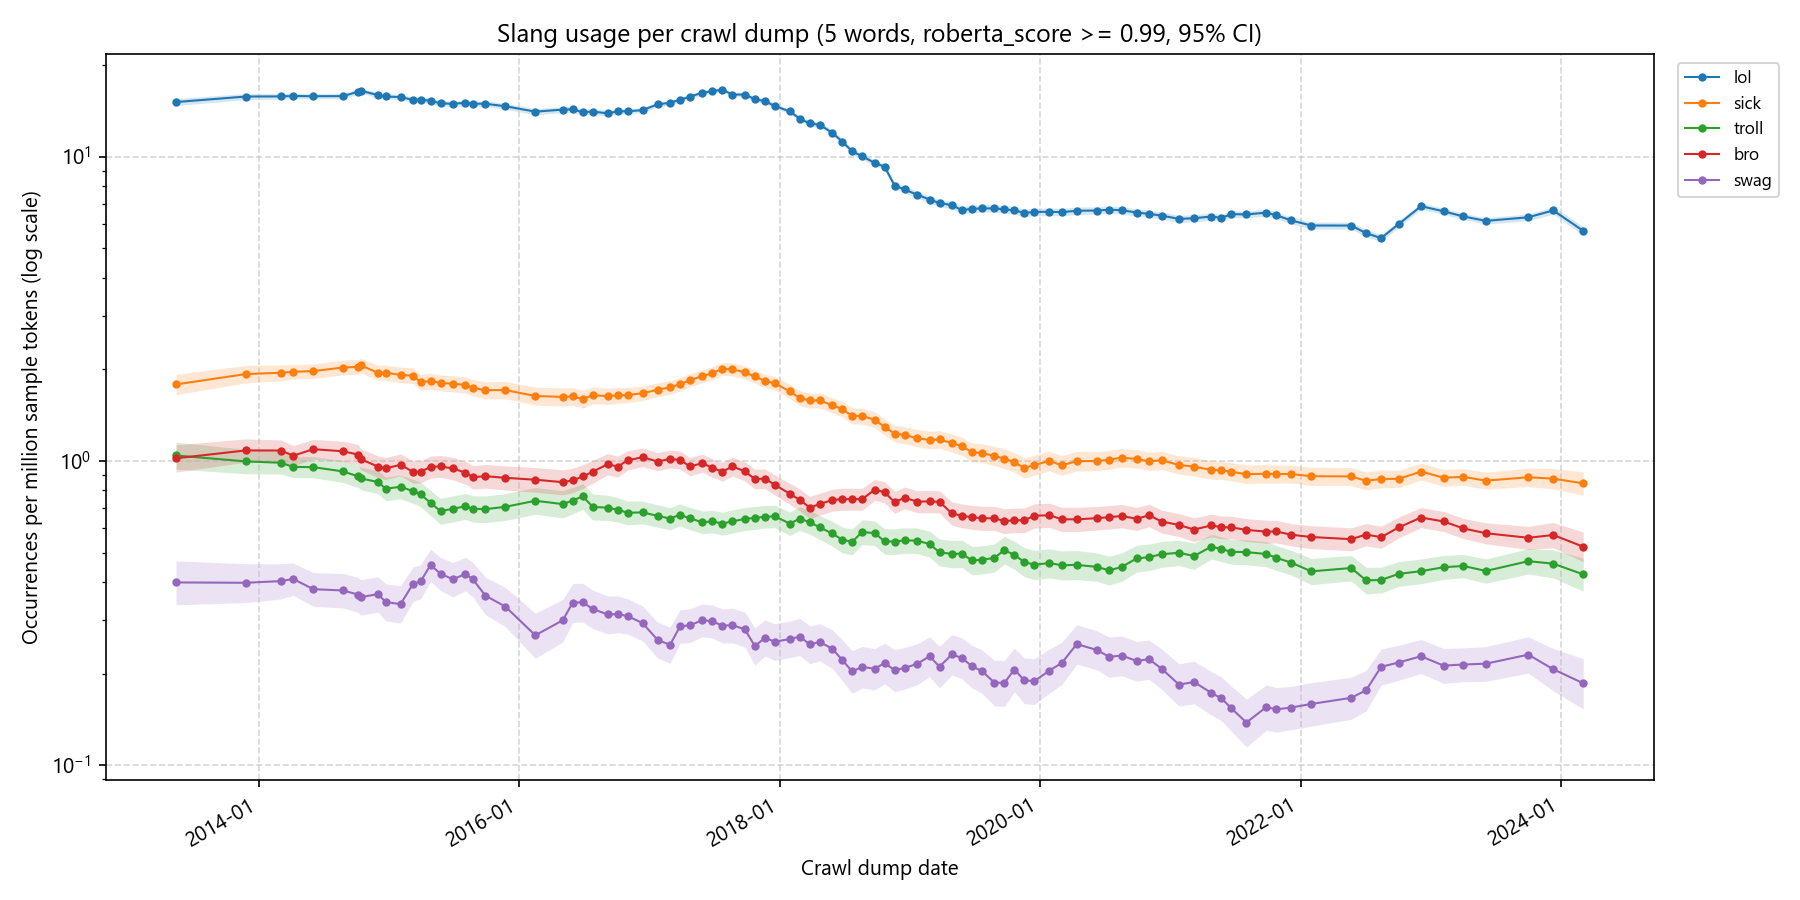
\includegraphics[width=1.0\linewidth]{highlight_pre2018.png}
    \caption{Slang-sense occurrences per million tokens by FineWeb crawl dump (log scale, RoBERTa score $\geq 0.99$, 95\% Poisson CI) for the pre-2018 band (\textit{lol, sick, troll, bro, swag}). \textit{lol} is the most frequent term throughout but declines steadily after $\sim$2018; \textit{swag} drifts downward, while \textit{sick}, \textit{troll}, and \textit{bro} are comparatively stable.}
    \label{fig:cc-pre2018}
\end{figure}

\begin{figure}
    \centering
    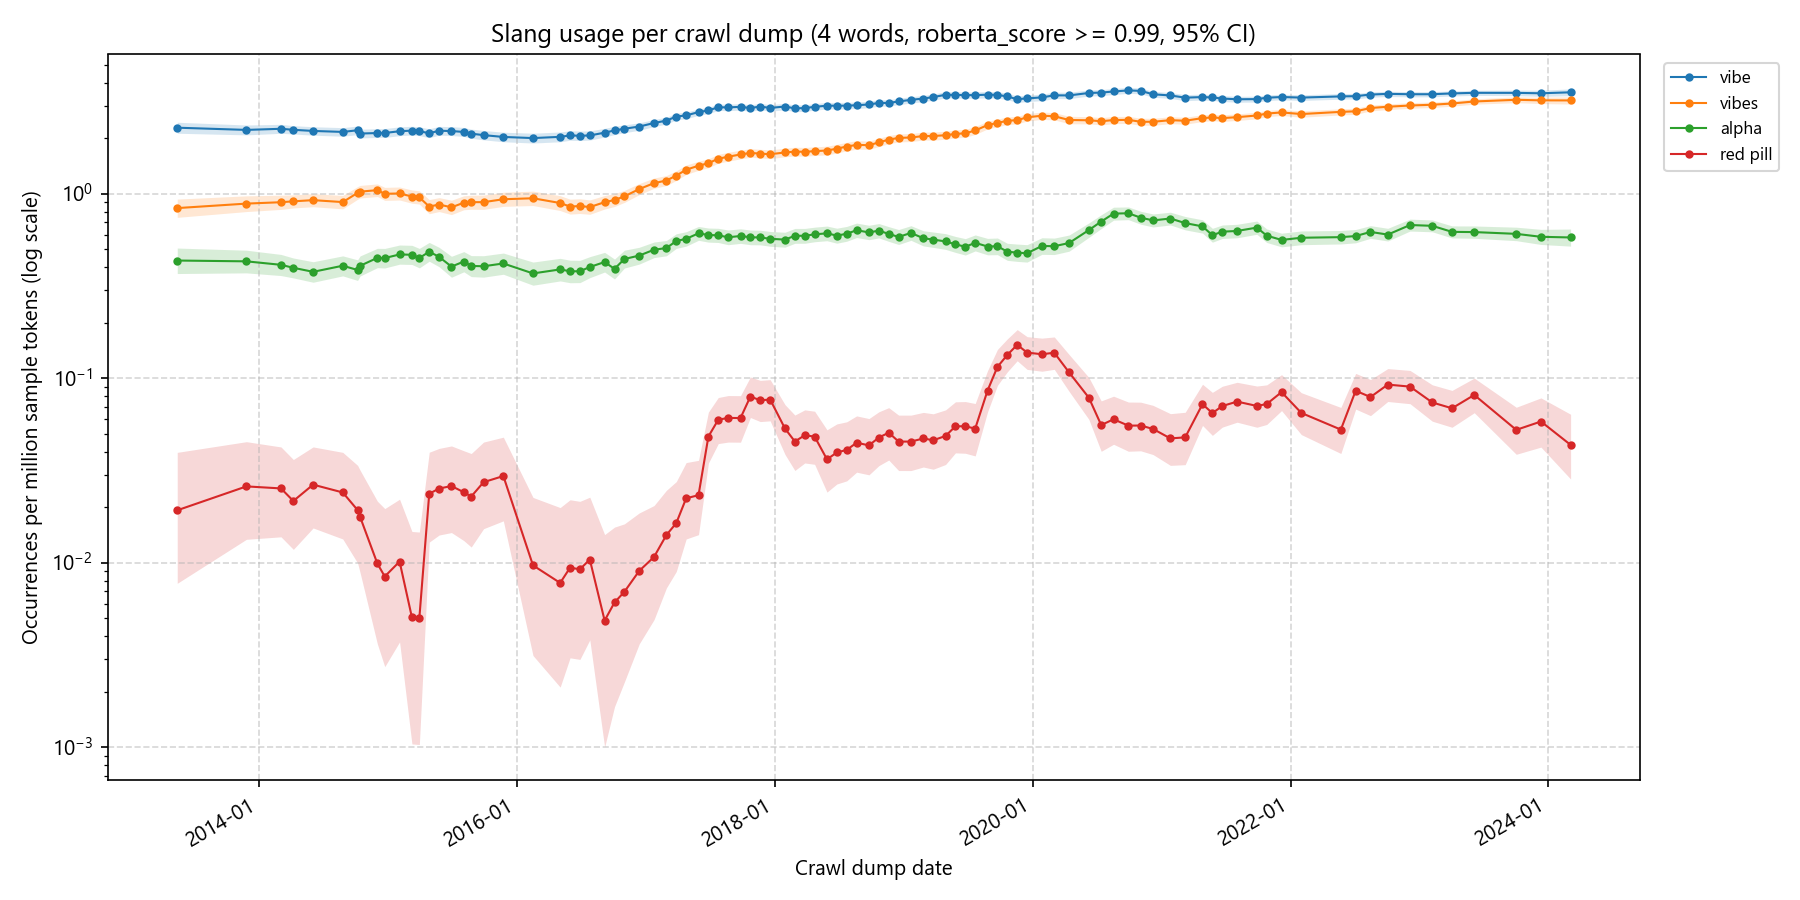
\includegraphics[width=1.0\linewidth]{highlight_around2020.png}
    \caption{Corpus frequency for the around-2020 band (\textit{vibe, vibes, alpha, red pill}). \textit{vibe} and \textit{vibes} rise through the late 2010s and into the 2020s; \textit{red pill}, a rarer and noisier term, sits well below with correspondingly wide confidence bands.}
    \label{fig:cc-around2020}
\end{figure}

\begin{figure}
    \centering
    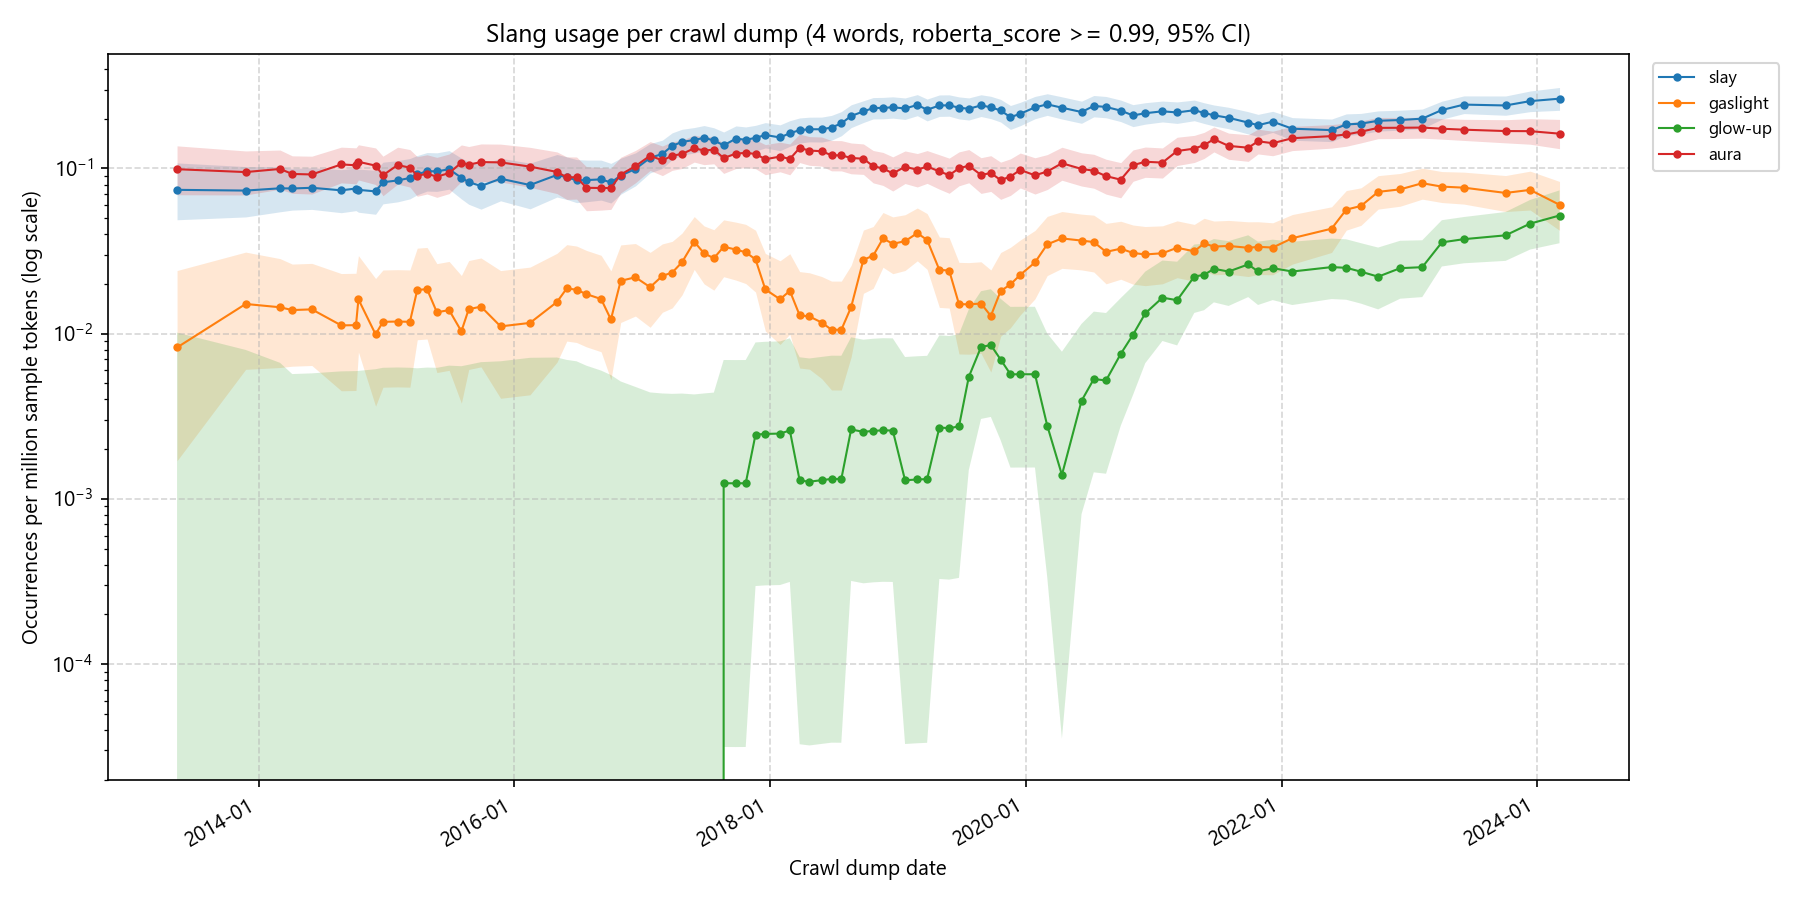
\includegraphics[width=1.0\linewidth]{highlight_2022_24.png}
    \caption{Corpus frequency for the 2022--2024 band (\textit{slay, gaslight, glow-up, aura}). These newest terms rise over the window, with \textit{aura} (in its Gen-Z slang sense) climbing sharply only near the end of the series --- the clearest example of slang that postdates the bulk of the models' training data.}
    \label{fig:cc-2022-24}
\end{figure}

Two properties matter for the probing analysis. First, the words we treat as ``older'' (\textit{lol}, \textit{swag}) are demonstrably in decline by the end of the window, while the ``recent'' words (\textit{aura}, \textit{slay}, \textit{glow-up}) are still rising --- so a model that reflected current usage would weight the latter group more heavily over time. Second, the sense filter is what makes these counts meaningful: without it, \textit{sick} and \textit{aura} would be dominated by their standard-English senses and show no slang lifecycle at all.

\todo{Extend the curves to the full set of available dumps and overlay each word's corpus peak year as a vertical marker, for direct visual comparison against the model-stated peak years in Experiment~4 (Section~\ref{sec:exp4}). Report the RoBERTa filter's held-out accuracy.}

\subsection{Experiment 2: LLM Output Probing}
\label{sec:exp2}

We report results for the three probing approaches. Approaches~1 and~2 below are \textbf{initial-attempt results} collected on \texttt{Llama-3.3-70B-Instruct-Turbo} and \texttt{Qwen2.5-7B-Instruct-Turbo} with an earlier candidate word set (\textit{lit}, \textit{fire}, \textit{rizz}, etc.); they are retained here as preliminary signal and are being re-run against the current four-model panel and the thirteen-word target set of Section~\ref{sec:exp1-method}. Approach~3 (Semantic Slot Probing) reports current results on all four models.

\subsubsection{Approach 1: Scenario-Based Generation (initial attempt)}

\textbf{Signal looks real, but sparse.} Only 45 total slang hits across 200 responses (0.23 per response), confirming the design risk: models default toward generic casual English and suppress overt slang. Not all prompts perform equally, the group chat prompt produced almost nothing, potentially can add more prompts that we think will perform better. \todo{Also check in llama (with RLHF) has a lower slang response rate.}

\begin{figure}
    \centering
    % \includegraphics[width=1.0\linewidth]{exp1.png} % TODO: figure not yet present in writing/
    \todo{Regenerate the scenario-generation slang-frequency bar chart for the current four-model panel and thirteen-word target set, and add the image to writing/.}
    \caption{Bar chart showing frequency of words from different slang eras in model responses (initial attempt).}
    \label{fig:barchart1}
\end{figure}

\textbf{Era bias is clear and significant.}
(See \hyperref[fig:barchart1]{Figure~\ref{fig:barchart1}})
\textit{lit} and \textit{fire} (2016--2019 era) dominate heavily. Nothing from 2023--2024 appeared at all (no \textit{rizz}, \textit{delulu}, \textit{brat},
\textit{NPC}). Initial experiment model cutoffs are late-2023, so we would expect to see some representation of slang popular from 2020-2023 at least.

\textbf{Prompt type matters substantially.} The text message scenario drove almost all slang (\textit{lit}$=$15, \textit{bae}$=$5, \textit{fleek}$=$2), while the group chat prompt produced zero. Scenario framing is important, make sure to investigate literature on prompt-response register effects and also remove poorer performing prompts and add some more ones that seem like they will perform well before a bigger test.

\textbf{Model split is observable.} A follow-up should disaggregate Llama vs.\ Qwen results to assess whether one model skews toward different eras. There's an expectation that Llama's use of RLHF discourages slang use in it's responses (cite, or do my own experiment if no cite. the logprobs experiment below already shows a large diff in some slang production between Qwen and Llama).

\subsubsection{Approach 2: Logprob Probing with Masked Templates (initial attempt)}

\textbf{\textit{lit} utterly dominates.} It is the top completion for 9 of 14 templates across both models, with some frames showing 98--99\% probability mass (\textit{``Bro that movie was \_\_\_''} $\to$ 98.9\%
Qwen, 53.4\% Llama; \textit{``The party last night was \_\_\_''} $\to$ 97.7\% Qwen, 82.1\% Llama). Of all era-tagged slang terms, \textit{lit} has 6$\times$ the average probability of the second-place finisher. We would expect this to map onto a correspondingly high prevalence of "lit" in the training data.

\textbf{The two models diverge meaningfully.} Llama defaults to \textit{awesome} for most generic frames, while Qwen uses for \textit{lit} in casual/contextual frames and produces subword token fragments in formal-sounding ones, this is fixed in iteration 2 where we collect multiple tokens from the experiment. Llama's relative aversion to using slang could be a product of the use of RLHF in it's training which has been shown to bias towards Standard American English (SAE) in responses \cite{barnhart2025rlhf}. \todo{Remove this whole first attempt from the results.}

\textbf{Register sensitivity is visible} Both models pick \textit{lit} for party/movie/show frames, but drift toward \textit{awesome} or \textit{electric} for \textit{``Their chemistry is \_\_\_''} and
\textit{``That speech was genuinely \_\_\_''}. This likely indicates the impact of prompt register and context on the behavior of models choice of language in responses.

\textbf{Nothing post-2020 appears at all} No \textit{bussin}, \textit{based}, \textit{goated}, \textit{rizz}, \textit{ate}. This needs to be confirmed that it's not a product of the model cutoff dates (which should be late 2023). Make sure that terms like "rizz" were seen in training data prior to 2023. Under our hypothesis we would expect to see some of these words used, just at a lower frequency more proportional to their occurrence in the training data.

\noindent\textit{Confound: subword tokenization artifacts (ep, aw, ro, cr) at max-tokens$=$1. A two-token follow-up pass resolves these.} \todo{Remove the initial busted experiment and consolidate the results with the multi-token followup.}

\paragraph{Multi-token follow-up}
\textit{lit} (2016--2019) is the dominant slang term --- top choice in 6 of 14 frames, averaging $P=0.78$. \textit{epic} (pre-2012) is the consistent pick for \textit{``Her comeback was \_\_\_''} on both models
($P=0.58$ Qwen, $P=0.63$ Llama). "Epic" is a word choice that has high representation in the full body of training data, but it's usage peaked in {year} and since {2020?} has show much less usage, especially compared to words that fill a similar linguistic slot such as "fire" and "lit".  Nothing post-2020 appears anywhere --- \textit{bussin, goated, rizz, ate, snatched} all have zero
presence even as low-probability alternatives, a strong signal across both experiments and both models. Confirm that this is represented by the training data, but if so these would both be good results for me hypothesis!

\begin{figure}
    \centering
    % \includegraphics[width=0.5\linewidth]{exp2.png} % TODO: figure not yet present in writing/
    \todo{Regenerate the masked-template logprob figure (per-model generated-word probability by era + first-token alternatives heatmap) on the two logprob-capable models, and add the image to writing/.}
    \caption{Masked-template logprob probing: probability mass on each candidate slang term by era (initial attempt).}
    \label{fig:experiment2chart}
\end{figure}

\subsubsection{Approach 3: Semantic Slot Probing}

The semantic-slot probe is run in two modes on the current four-model panel. In the \textit{concept-slot} mode the model is given a temporally neutral definition of a meaning (``cool/impressive'', ``mediocre'', ``charisma'', ``suspicious'', \dots) and asked for a single informal word, surfacing whatever era of slang the model reaches for. In the \textit{target-recovery} mode the definition is written to point at one specific target word, and we measure how often the model returns that exact word (allowing inflections and stem matches) --- a direct measure of how reluctant the model is to produce the intended slang term, and of whether the term is effectively out of vocabulary.

\textbf{Target-recovery accuracy varies sharply by word, not just by model.} Figure~\ref{fig:slotaccuracy} shows, for each target word, the percentage of responses that recovered the intended word, one bar per model (ten samples per phrasing, three phrasings per word). Aggregate recovery is highest for \texttt{claude-sonnet-4-6} (71\%), followed by \texttt{gpt-4o} (62\%) and \texttt{DeepSeek-V4-Pro} (60\%), with \texttt{Llama-3.3-70B} lowest at 53\% --- consistent with RLHF-driven slang suppression in the Llama model. Unambiguous, well-established terms (\textit{lol}, \textit{troll}, \textit{gaslight}, \textit{glow-up}) are recovered near-perfectly by every model, whereas polysemous or contested slots are hard across the board: \textit{sick} (models answer the literal ``awesome''/``cool'' rather than the slang \textit{sick}), \textit{swag} (models prefer the competing \textit{swagger}/\textit{drip}), and the most recent term \textit{aura} (models reach for \textit{clout}, \textit{charisma}, or \textit{vibe}) are recovered well below a third of the time for most models.

\textbf{The hardest slots are the most diagnostic.} That \textit{aura} --- the newest term, still sharply rising in the corpus (Figure~\ref{fig:cc-2022-24}) --- is the word models are least able to produce on demand is consistent with the central hypothesis: the slang that is most current in human usage is the slang the models are least fluent in. Conversely, the words recovered most reliably are the older, well-attested terms that have saturated the training data.

\begin{figure}
    \centering
    
\includegraphics[width=1.0\linewidth]{target_word_accuracy.png}
    \caption{Semantic-slot target-word recovery accuracy. For each target word (x-axis, in rough chronological order of peak usage) the bars give the percentage of responses, per model, that returned the intended word (stem/inflection matches counted). Older, unambiguous terms are recovered reliably; polysemous (\textit{sick}, \textit{swag}) and very recent (\textit{aura}) terms are recovered poorly.}
    \label{fig:slotaccuracy}
\end{figure}

\paragraph{Concept-slot mode (initial attempt).} The following observations are from the earlier two-model concept-slot run and are being folded into the current panel.

\textbf{"Mediocre" slot is the sharpest result}
Both models independently converge on \textit{meh} across 3 of 4 phrasings with very high confidence (logprobs of $-0.01$ to $-0.04$, $\sim$99\% probability). \textit{meh} is pre-internet in origin but became widely web-native via
\textit{The Simpsons}.
\todo{meh is not in our target word set, we can add it if it hold as a good example in the training data analysis, which I think it might. It's not very commonly used anymore, but used to be a pretty popular word online.}

\textbf{Cool/impressive slot shows the model split most clearly.} Qwen reaches for \textit{rad} (pre-2012) and \textit{lit} (2016--2019) roughly equally; Llama defaults to \textit{awesome} for 3 of 4 phrasings. Neither touches anything post-2020. Llama's use of "awesome" is likely due to RLHF causing it to avoid slang more than other models. This could be tested when we use a larger selection of models in experiment. We could also try re-running against the Llama base model (pre-RLHF) and see how that changes the results.

\textbf{Charisma slot is the most interesting divergence.} Both models produce \textit{swag} (a 2012--2015 term), but \textit{rizz} --- the 2023 Oxford Word of the Year that fills exactly this semantic slot ---
appears nowhere, not even as a low-probability alternative. \todo{If the bias is actually caused by data dilution rather than cutoff behavior, then we should at least see SOME use of rizz, especially given how frequently it is used online.}

\textbf{Suspicious slot has the best slang coverage.} \textit{sketchy}, \textit{shady}, \textit{fishy}, and \textit{sus} (2020--2022) all appear. Qwen surfaces \textit{sus} as a first-token alternative at
20.7\% --- the only 2020+ slang term to show meaningful probability mass across any experiment. \todo{This needs to be rerun, since these prompts were also affected by containing slang words, sketchy and shady were actually used in the prompts so... if it hold with cleaner prompts though sus def became a thing in 2020 during those amogus days. Noteably, the other no occurence examples are much later even, 2023. So we'd estimate the "true" cutoff date here to be sometime in 2020-1 based on this finding. Should compare this to the findings from the cutoff paper to see if they match.}

\begin{figure}
    \centering
    % \includegraphics[width=1.0\linewidth]{exp3.png} % TODO: concept-slot figure not yet present in writing/
    \todo{Regenerate the concept-slot figure (per-slot word tiles coloured by era + per-era probability-mass summary) for the current four-model panel, and add the image to writing/.}
    \caption{Concept-slot probing: words produced per semantic slot, coloured by era of peak usage (initial attempt).}
    \label{fig:experiment3graph}
\end{figure}

\subsection{Experiment 4: Direct Year Association}
\label{sec:exp4}

Experiments~1--3 measure what slang the models \textit{use}. Experiment~4 instead asks what the models \textit{know} about slang timing, by posing the temporal question directly (Section~\ref{sec:exp4-method}). The contrast is the key result: the models carry \emph{directionally} correct declarative knowledge of when slang was popular --- they order terms by era far better than chance --- yet that knowledge is both noticeably shifted toward the past and not reflected in their spontaneous usage (Experiments~2--3).

\textbf{The figure overlays model belief against corpus ground truth.} Figure~\ref{fig:yearassoc} places the target words on the y-axis \emph{ordered by their true corpus peak year} (from Experiment~1), with calendar year on the x-axis. For each word a red star marks the corpus peak and a dark diamond marks the model's mean responded year, pooling the \textit{GiveYear} and \textit{DatePhrase} samples; the line connecting them is the model's error, and the faint points show the spread of individual responses. Because the words are sorted by true peak, the stars form a rising staircase, so the horizontal offset of each diamond from its star reads directly as how far the model is off.

\textbf{Models order slang roughly by era but compress it toward the past.} The diamonds broadly follow the staircase --- models do place \textit{lol}, \textit{troll}, and \textit{bro} early and \textit{aura} and \textit{slay} late --- but they systematically date the newer terms too early. For \texttt{claude-sonnet-4-6}, \textit{alpha} (corpus peak 2020) is placed near 2010, and \textit{vibe}/\textit{vibes} (still rising through 2024) near 2018/2020. The mean absolute error against the corpus peak is sizeable for every model: 6.2 years for Claude, 7.7 for Llama, and 8.0 for DeepSeek, consistent with a sense of slang anchored to an earlier window than current usage.

\textbf{Caveat on the comparison.} The corpus ``peak'' is the year of maximum frequency, so for the words still rising at the end of the data window (2023--2024 peaks) it is closer to a lower bound on recency than a true crest; a model dating \textit{vibe} to 2018 is arguably reporting the \emph{onset} of popular use rather than the corpus peak. The comparison is cleanest for words that have visibly crested within the window (\textit{lol}, \textit{swag}, \textit{alpha}), where the models still skew early. \texttt{gpt-4o} is a special case: its lower 4.4-year error is an artifact rather than better calibration, since its \textit{DatePhrase} responses collapse to ``2023'' (the apparent present) for almost every word, which happens to sit near the many recent peaks.

\begin{figure}
    \centering
    
\includegraphics[width=1.0\linewidth]{give_year_date_phrase_claude.png}
    \caption{Direct year association for \texttt{claude-sonnet-4-6}, pooling the \textit{GiveYear} and \textit{DatePhrase} prompts. Words (y-axis) are ordered by their true corpus peak year (Experiment~1, shown in parentheses); the x-axis is calendar year. For each word the red star is the corpus peak, the dark diamond is the model's mean responded year, the connecting line is the error, and faint dots are individual responses; markers falling outside 2010--2024 are drawn as arrows at the axis edge. The diamonds track the rising staircase of true peaks only loosely and skew early for the newer terms (mean absolute error 6.2 years). Per-model figures for \texttt{gpt-4o} (4.4 yr, inflated by its collapse to ``2023''), \texttt{DeepSeek-V4-Pro} (8.0 yr), and \texttt{Llama-3.3-70B} (7.7 yr) are included as supplementary figures (\texttt{give\_year\_date\_phrase\_*.png}).}
    \label{fig:yearassoc}
\end{figure}

\textbf{Interpretation.} Even granting the onset-vs-peak caveat, the picture refines rather than overturns the central claim. The models possess \emph{directional} temporal knowledge --- they order slang by era far better than chance --- but that knowledge is both compressed toward the past and, critically, not reflected in their actual usage (Experiments~2--3). The failure to produce current slang is therefore not a total absence of temporal knowledge, but a usage bias compounded by a backward-shifted sense of when ``recent'' slang belongs.

\todo{Add the \textit{AssociateSlangLogprobs} association-surface heatmap for the open models, and report per-word error against the corpus peak rather than only the aggregate MAE.}

% ============================================================
\section{Results}

Findings from the corpus analysis and the probing experiments converge on a consistent pattern:

\begin{itemize}
  \item \textbf{The target words have genuine, separable lifecycles.} The corpus analysis (Experiment~1, Figures~\ref{fig:cc-pre2018}--\ref{fig:cc-2022-24}) confirms that the older terms (\textit{lol}, \textit{swag}) are in decline by the end of the window while the newest terms (\textit{aura}, \textit{slay}, \textit{glow-up}) are still rising. This is what makes the words usable as a temporal probe and validates the curated target set.

  \item \textbf{Models are least fluent in the most current slang.} In semantic-slot recovery (Experiment~3, Figure~\ref{fig:slotaccuracy}), every model recovers older, unambiguous terms (\textit{lol}, \textit{troll}, \textit{gaslight}, \textit{glow-up}) near-perfectly, but recovery collapses for the newest term \textit{aura} and for polysemous slots (\textit{sick}, \textit{swag}) where the model prefers a competing or literal word. The slang that is most current in human usage is the slang the models are least able to produce on demand.

  \item \textbf{Knowing-when and using-now come apart.} The year-association probes (Experiment~4, Figure~\ref{fig:yearassoc}) show that models order slang by era directionally correctly, but place the newer terms years too early relative to the corpus peak (mean absolute error 6--8 years per model), and their spontaneous usage does not track recency at all. The temporal failure is thus a usage bias on top of a backward-shifted, rather than absent, sense of slang timing.

  \item \textbf{Model-level differences are consistent with RLHF slang suppression.} \texttt{Llama-3.3-70B} has the lowest semantic-slot recovery (53\% vs.\ 71\% for Claude) and most readily defaults to neutral standard-English words, consistent with reports that RLHF biases toward Standard American English \citep{barnhart2025rlhf}. \texttt{gpt-4o} exhibits a distinct artifact --- collapsing \textit{DatePhrase} answers to the present year --- that is orthogonal to the era bias but worth noting. \todo{Confirm whether DeepSeek/Claude RLHF pipelines differ enough to explain the recovery-rate spread.}
\end{itemize}

\todo{Re-run the scenario (Approach 1) and masked-logprob (Approach 2) probes on the current four-model panel and target-word set, and overlay the Experiment~1 corpus peak years on the Experiment~4 estimates for a direct ground-truth-vs-belief comparison.}

% ============================================================
\section{Discussion}

\subsection{Interpretation}

Results suggest the models do not display temporal sensitivity in their spontaneous slang usage --- when asked to produce current slang on demand they reliably return older, well-attested terms and struggle most with the newest ones (Experiment~3) --- even while they retain accurate declarative knowledge of when those terms were popular (Experiment~4). This is consistent with the hypothesis that model slang \textit{usage} reflects total frequency in the training corpus rather than a temporally calibrated view of what is current. \todo{Add some more comments and citations here about the importance of slang and language evolution. AKA why does this isolated effect matter, even if you don't agree with my downstream implications section.}

The difficulty models have producing the most recent term \textit{aura} --- still sharply rising in the corpus at the end of the window --- is striking precisely because the same models date it to roughly the right era (2023--2024) when asked directly (Figure~\ref{fig:yearassoc}). \textit{aura} is the cleanest illustration of usage-bias-without-a-knowledge-gap: the model knows when the word belongs yet will not produce it on demand. For most other recent terms the model additionally shifts its stated date years too early, so the two effects --- backward-shifted belief and a usage bias on top of it --- compound. The reliability gap between recovering older versus newer slang may reflect that the older terms have saturated the training data with strong, redundant signal, whereas the newest terms appear in quantities too small (and too close to the data-collection horizon) to anchor confident generation, despite being the dominant form in current human usage.

\subsection{Implications for Training Data}

If LLMs cannot naturally update their vocabulary with the pace of language change, this creates a compounding problem as internet text becomes increasingly LLM-generated \citep{shumailov2023curse}. LLM-generated text will continue to reflect frozen, older vocabulary, potentially poisoning future corpora and further reducing models' capacity to reflect current human language. This also provides a similar critique to the broader ``stochastic parrots'' concept \citep{bender2021parrots}: models learn structure from language but may not generalize to dynamic linguistic change. \todo{Claude said this and idk if it makes sense or not... do we want to say that this provides further evidence for concerns raised in parrots? Or do we also want to say that these results demonstrate lack of reasoning? What?} Currently, this may have a small effect on model responses, especially due to preferences against slang use (see Llama's RLHF effect).
However, these results indicate that generational language shift may be similarly effected, which may have a larger and more problematic impact. If language models persist for the next 100 years, what will the language they generate look like? Will it be rooted in the average of what human-generated data we have from 125 years of collection? In that case, these results indicate that we may have models producing language many decades out of date from real-world usage. In order to maintain relevant and reflective vocabulary in models, this problem will need to be addressed through model training interventions (recency sampling) and continual availability of up-to-date human generated language for training.

This provides a strong argument in favor of verifiably human-generated text as a premium training resource.

% ============================================================
\section{Limitations}

\subsection{Does Prompt Language Condition the Response?}

One limitation to acknowledge: if a user prompts in contemporary 2025 English, does that effectively condition the model's output toward more current vocabulary? If so, the practical impact of temporal vocabulary drift may be lower than the probing experiments suggest.

\todo{Literature review to assess whether prompt register effectively conditions output register/vocabulary. Presumably it does.}

\begin{itemize}
  \item Model comparison across cutoff dates is confounded by architectural differences. E.g. RLHF
  \item Logprob access may be limited to top-$k$ tokens, constraining probing methodology.
  \item Much internet slang is appropriated AAVE; this linguistic and cultural dimension is not fully addressed here. But bias in models against non-standard English has been observed \cite{barnhart2025rlhf}.
  \item Common Crawl upsampling (seen in Dolma model, and maybe others that we don't have access to) may distort raw frequency analysis.
  \item All four probed models (Llama-3.3-70B-Instruct-Turbo, DeepSeek-V4-Pro, gpt-4o, claude-sonnet-4-6) are instruction-tuned. RLHF and instruction tuning may suppress slang relative to base models, potentially amplifying the apparent temporal freeze; replicating on base models would isolate this.
  \item Logprob-based probes (Approach~2; \textit{AssociateSlangLogprobs}) run only on the two open-weight models, since the closed APIs do not expose token logprobs; closed-model distributions are approximated by repeated sampling, which is noisier.
\end{itemize}

\todo{Revisit this section after experiments to add any additional limitations surfaced during.}

% ============================================================
\section{Future Work}

\subsection{Stretch Experiment: Fine-tuning as Mitigation}

We plan to investigate whether fine-tuning on a recent-only data subset can shift the model's vocabulary toward more contemporary usage.

\begin{itemize}
  \item \textbf{Approach:} fine-tune on a subset of the most recent
  Common Crawl dumps only; re-run probing experiments.
  \item \textbf{Sub-question:} does fine-tuning on a duplicate subset of data change usage patterns at all? (Essentially try upsampling based on recency.)
\end{itemize}

Additional ideas for future expansion of this work are:
\todo{ Review literature on recency-weighted training / continual
learning for LLMs.}
\begin{itemize}
  \item Expanded fine-tuning experiments with recency-weighted corpora.
  \item Longitudinal study: retrain models on successive Common Crawl
  snapshots and track vocabulary drift over time. Way too expensive for the scope of this project, since it would involve pretraining models.
  \item Investigating sub-year temporal resolution --- can models distinguish slang peaks within a single year (e.g., the ``Ohio'' meme)?
  \item Replicating probing experiments on base (non-instruction-tuned) models to isolate RLHF effects on slang suppression. This also might already exist in the literature.
\item Multilingual analysis of temporal vocabulary drift.
  \item The implications in multi-lingual settings could be very different. It would be interesting to find our how low resource (low training data) languages are affected by this. Is it more, because model generated language could quickly overtake human generated examples for less resourced languages? Or less because languages with less training data are more easily influenced by more recent data?
\end{itemize}

% ============================================================
\section*{Acknowledgments}
\todo{Fill in acknowledgments before camera-ready submission.}

% ============================================================
\bibliography{references}

\appendix{Appendix}
\begin{lstlisting}[language=json, caption={Scenario-based generation prompt templates (Experiment 1).}, label={lst:exp1-prompts}]
{ "id": "exp1_text_message",
  "system": "Write informally, exactly the way people type in real
             text messages. Output only the message text.",
  "user": "Write a text message from a teenager to their friend
           about {event}.",
  "variables": {
    "event": [
      "a party they went to last weekend",
      "a concert they just got back from",
      "something wild that happened at school today",
      "seeing someone get dramatically rejected in front of everyone",
      "a house party that got out of hand"
    ]
  }
}

{ "id": "exp1_reddit_comment",
  "system": "Write exactly the way people comment on Reddit.
             Informal, direct -- just the comment text.",
  "user": "Write a Reddit comment reacting to this hot take:
           \"{hot_take}\"",
  "variables": {
    "hot_take": [
      "The Dark Knight is overrated",
      "Pineapple on pizza is actually good",
      "Video games are a waste of time",
      "Pop music is better than it has ever been",
      "Sequels are almost always worse than the original"
    ]
  }
}
\end{lstlisting}


\end{document}
